\documentclass[11pt]{article}
\usepackage{fullpage}
\usepackage{setspace}
\usepackage{amsmath}
\usepackage{fancyvrb}
\usepackage{enumerate}
\usepackage{listings}
\usepackage{pgfplots}
\usepackage{graphicx}
\usepackage{float}
\usepackage{multirow}
\usepackage[format=hang,labelsep=quad]{caption}
\usepackage{subfig}
\usepackage{array}
\usepackage{multirow}
\usepackage[final]{pdfpages}

\renewcommand\thesubfigure{\roman{subfigure}}


\begin{document}
\noindent\large{Math 5364}\\
\large{Data Mining 2}\\
\large{Homework 29}\\
\large{Mary Barker}

\begin{Verbatim}
*1. Import the file math5305Lab6Data.txt, whose columns are the 
	variables Y, X_1, X_2, X_3. In Homework 27, we saw that the 
	model 
	
		Y = beta_0 + beta_1 X_1 + beta_2 X_2 + beta_3 X_3 + e

	does not satisfy the assumption e_i ~ N(0, sigma^2),i=1,...,n
	To remedy this, preform a Box-Cox transformation of Y by defining 

		tildeY_i = ((Y_i)^lambda - 1) / lambda for i = 1, ... , n;

		options obs=100;
		
		data problem1;
		    infile '/folders/myshortcuts/sas_folder/math5305Lab6Data.txt' dlm=',';
		    input Y X1 X2 X3;
		run;

	*a. Fit the model 
		tildeY = beta_0 + beta_1 X_1 + beta_2 X_2 + beta_3 X_3 + e
		
		and let hat_tildeY and tilde_e be the predicted values and 
		residuals for this transformed model;

		proc transreg data=problem1 detail(NOKNOTS NOCOEFFICIENTS);
			model boxcox(Y/lambda = -2 to 2 by .01) = Identity(X1 X2 X3);
			output out=myoutput;
		run;
		proc reg data=myoutput;
			var TY TX1 TX2 TX3;
			model TY=TX1 TX2 TX3;
			output out = transformed_model_output
				predicted=hat_tildeY
				residual=tilde_e;
		run;

	*b. Plot tildeY vs hat_tildeY and tilde_e vs. hat_tildeY. Does 
		curvature appear to exist in the transformed model? ;

		proc plot data=transformed_model_output;
			plot Y * hat_tildeY
				 tilde_e * hat_tildeY;
		run;
		
	*c. Investigate normality of the errors for the transformed model;

		proc univariate data=transformed_model_output normal;
			var tilde_e;
			qqplot tilde_e;
		run;


	*d. Investigate constancy of error variance for the transformed 
		model;

		proc reg data=transformed_model_output;
		    model TY=TX1 TX2 TX3/SPEC;
		run;


	*e. Do the errors for the transformed model appear to satisfy the 
		assumptions of normality and constant error variance? How do 
		your results compare to those of Homework 23? ;



*2. The file math5305Lab7Data.txt contains data contains data for the 
	variables Y, X_1, X_2, ... , X_40. Perform a stepwise regression 
	on this data set using SAS. (Hints: It may be helpful to use the 
	"import data' option in the "file" menu to import this data. Also, 
	make sure to specify in your glemselect procedure which variables 
	are class variables. Finally, it may be convenient to use R to 
	generate the model statement for this procedure.);


		options obs=2000;
		data problem2;
		    infile '/folders/myshortcuts/sas_folder/math5305Lab7Data.txt' dlm=',';
		    input Y X1 X2 X3 X4 X5 X6 X7 X8 X9 X10 X11 X12 X13 X14 X15 X16
		    		X17 X18 X19 X20 X21 X22 X23 X24 X25 X26 $ X27 X28 X29 X30
		    		X31 X32 X33 $ X34 X35 X36 X37 X38 X39 X40 $;
		run;
		proc glmselect data=problem2;
			class X26 X33 X40;
			model Y = X1-X40 / selection=stepwise ;
			output out = stepwise_results;
		run;


\end{Verbatim}
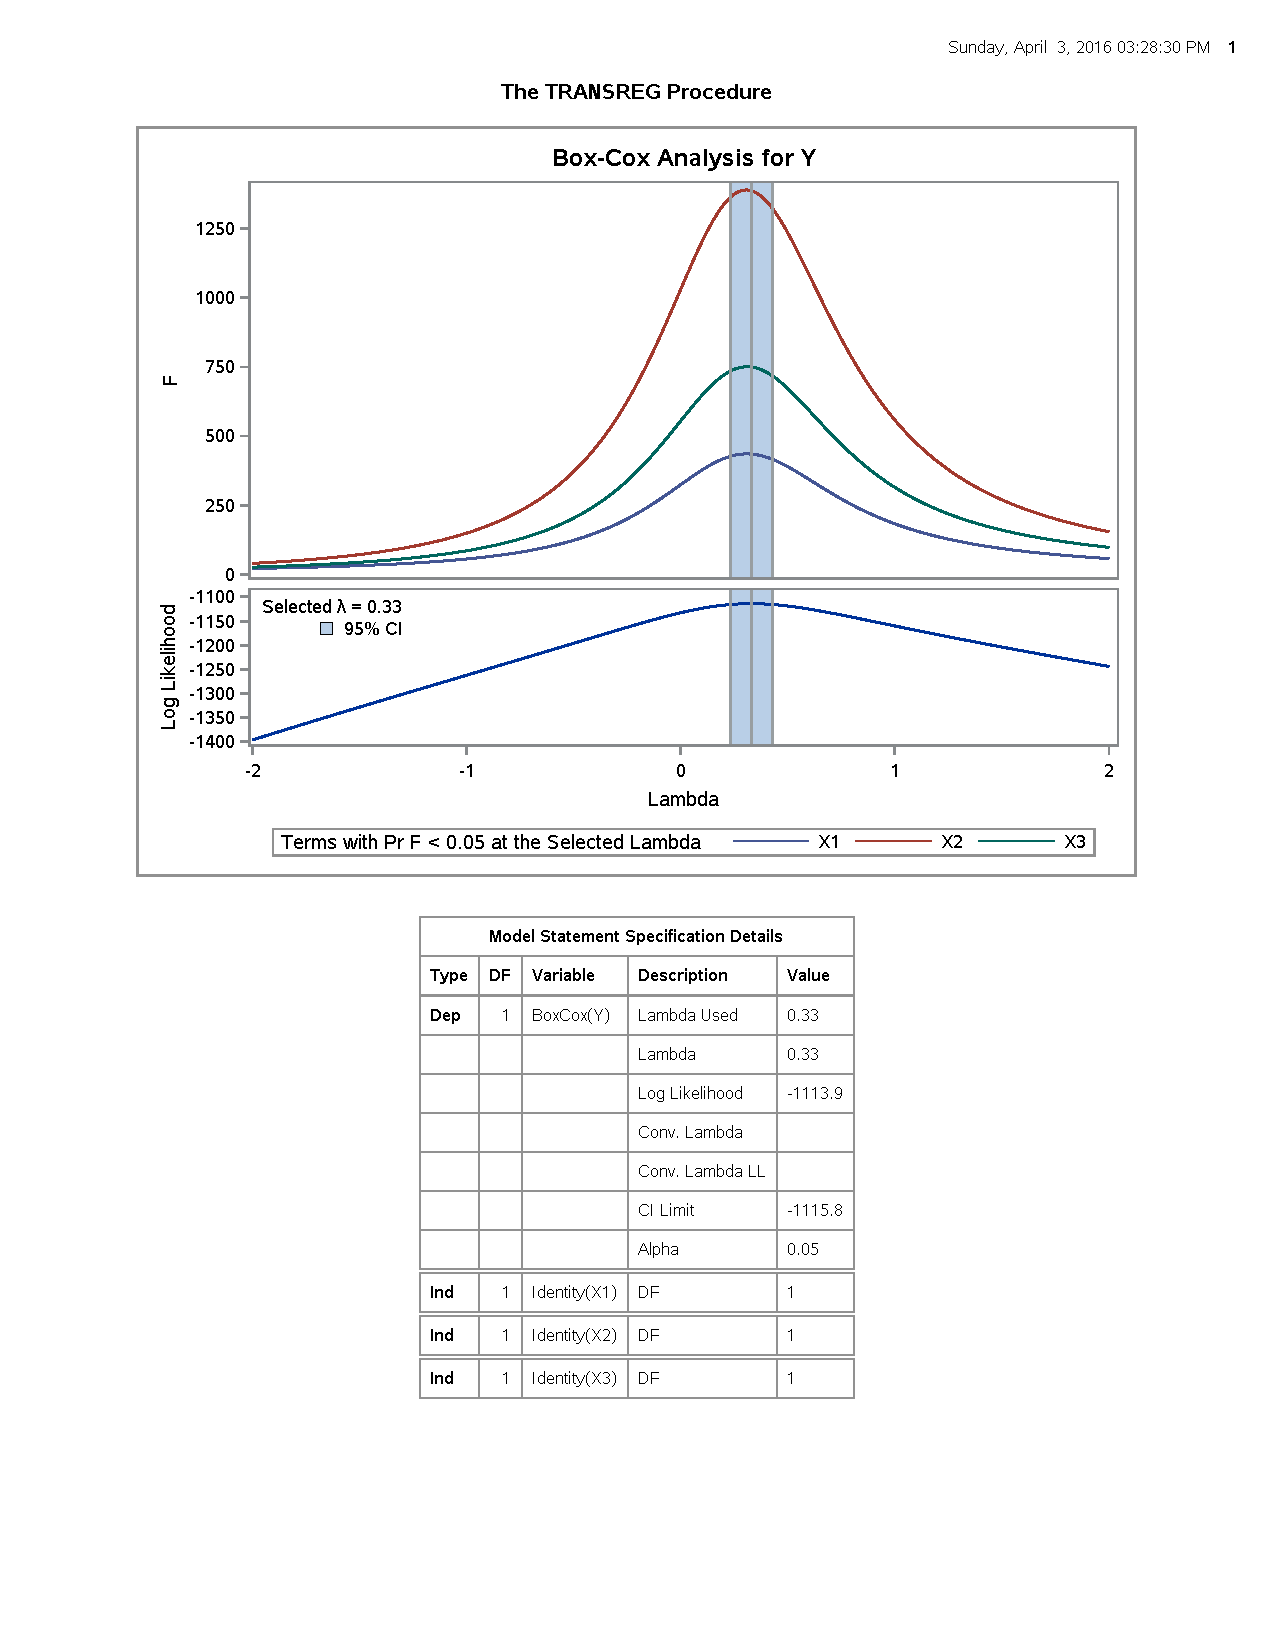
\includepdf[pages={1-}]{hw29-results.pdf}
\end{document}
